%!TEX root = /Users/simo/Documents/PFC/memoria/memoria.tex

\section{Planificación} % (fold)
\label{sec:planificacion}
El paso natural en el proceso de desarrollo de esta aplicación según las metodologías típicas sería realizar toda una etapa de diseño desde la cual se realizarían todos los diagramas correspondientes a su futura implementación. Sin embargo, y como se explicará en la sección de desarrollo, para esta aplicación se seguirá una metodología de desarrollo ágil, muy común en los entornos de desarrollo web.

Dichas metodologías defienden un desarrollo iterativo, que incluye todas las etapas (incluyendo el diseño) en cada iteración. No obstante, es necesaria una mínima planificación, especialmente para la parte de la pizarra, la cual es prácticamente independiente del resto, y por las características de Javascript hace difícil realizar un desarrollo completamente formal.

\subsection{Pizarra}
Se ha explicado con anterioridad las características de Javascript, el cual, a pesar de sus limitaciones, es orientado a objetos, y es posible programar de forma bastante modular gracias a ello. 

El código que manejará los elementos de la pizarra se distribuirá en una serie de módulos. Hay que recordar que la Pizarra está integrada en un sistema, que es la página web, que le proveerá con la información necesaria. Por ejemplo, Javascript de por si no es capaz de consultar una base de datos, pero si consultar otra página mediante Ajax, que le devuelva lo que necesita saber. Dicha página será generada por el \textbf{Sistema}, que en este caso funcionará bajo Ruby on Rails, que será el que consultará la base de datos y genere los datos con el formato adecuado para que Javascript lo pueda entender. Se puede observar la figura \ref{fig:javascript-data} a modo de ejemplo explicativo del proceso.

\begin{figure}[h]
\centering
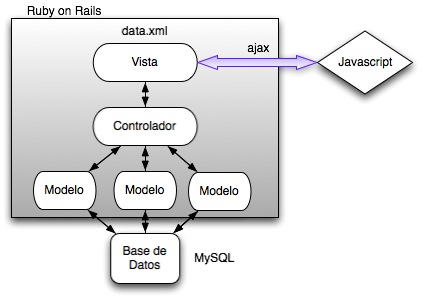
\includegraphics{javascript-data.jpg}
\caption{Esquema de la obtención de datos mediante javascript}\label{fig:javascript-data}
\end{figure}


\begin{description}
	\item[Renderizado] Aquí se agruparán las funciones que dibujen los elementos. Debe tener las funciones necesarias para poder dibujar los elementos que se soporten (líneas, polilíneas, cuadrados, círculos, etc), así como editarlos, y que sea capaz de hacerlo independientemente del navegador que se esté usando.
	\item[Dibujo] Será el módulo que controle los eventos del ponente. Debe ser capaz de entender los movimientos de ratón y teclado de forma que indique al módulo de renderizado las figuras que debe crear de forma que se experimente una sensación de dibujo interactivo. Además, debe utilizar el módulo de comunicación para informar al sistema cuándo se ha creado, editado, o eliminado algún elemento.
	\item[Comunicación] Éste módulo incluirá las funcionalidades de comunicación entre la interfaz, en javascript (recordando que javascript es incapaz de consultar bases de datos), y el sistema web. Será capaz de informar en ambas direcciones, tanto cuando el ponente ha modificado la pizarra para decírselo al sistema, como cuándo el sistema recive nuevos elementos, para comunicárselos a los espectadores.
\end{description}

Debido a las características peculiares de Javascript, se considera este enfoque como el más sencillo y eficiente para un programador con conocimientos escasos del lenguaje. El hecho de que javascript sea orientado a objetos, permite que se creen clases adecuadas para poder representar las clases del dominio, sin embargo, sigue siendo más sencillo implementar dichos controladores como una serie de funciones agrupadas en un archivo, más que hacer realmente una clase Renderizado, con subfunciones. En cualquier caso, se dará una gran importancia a intentar implementar de forma coherente con el paradigma de orientación a objetos, en la medida de lo posible acorde con las características de Javascript, y el nivel de conocimiento del lenguaje del programador. En esta fase del desarrollo es difícil definir hasta qué punto será posible.


\subsection{Sistema}

El sistema debe servir como intermediario entre todos los usuarios que participan en una pizarra, y ser capaz de realizar las funciones que Javascript, de por si solo, no es capaz. Antes de empezar a participar en alguna pizarra hay una serie de acciones que deben de ser controladas por el sistema. Dichas funcionalidades se pueden recoger en una serie de módulos, los cuales más adelante se intentarán formalizar en una estructura compatible con el paradigma Modelo-Vita-Controlador de Rails.

\begin{description}
	\item[Control de Usuarios y Grupos] Es necesario mantener un control de los usuarios y los grupos a los que se pertenece, y para ello es necesario una base de datos. Los usuarios tienen que poder registrarse y hacer las funciones típicas, como Login, edición de datos, creación de grupos, etc. Éste módulo debería ser capaz de controlar todo lo referente a usuarios y grupos según el comportamiento que se ha definido anteriormente.
	\item[Control de Pizarras] Las responsabilidades de este módulo serían las de mantener un control de las pizarras que existen, sus permisos, y su contenido. Cada pizarra tiene una serie de páginas, y cada página una serie de elementos, que deben de ser accesibles y modificables, así como poder crear o eliminar nuevos.
	\item[Comunicación con Javascript] Ésta es la funcionalidad más importante, y a falta de un nombre más apropiado, este módulo debe hacer precisamente esto, ser capaz de comunicarse con la interfaz, que se está ejecutando en el cliente, y no en el servidor. Debido a las características de Ajax y de Rails, se cree que no será posible separar formalmente estas funcionalidades, y que deberá ser incluida en los otros dos módulos.
\end{description}